%-------------------------------------------------------------------------------
\section{Evaluation}
%-------------------------------------------------------------------------------
\kam{I haven't worked fleshed out this section. It is basically just all the stuff I need to talk about} \newline
\kam{WIP: To strengthen the eval, I'm implementing a straw-man for graph representations as a baseline to compare our technique against} \newline

For our evaluation, we obtained traces from a large e-commerce company, where the underlying system is a micro-service architecture. The traces encapsulate the request-response interactions of micro-services. We obtained traces from three different request paths in the system that correspond to viewing, selling and checking out an item in the catalog. The request paths are not mutually exclusive i.e. they share some services\kam{TODO: How many shared services?} and traces from the same request path can vary subtly based on the exact request parameters.

We use graphs corresponding to a small fraction of traces\kam{TODO: How many?} are used to generate node representations which are then used by clustering, prediction and diagnostic tasks. 

Sanity check: 
\begin{itemize}
\item Compute representations for all graphs
\item Cluster graph representations
\end{itemize}
Use Adjusted-Rand index to compare expected labels with obtained labels

Adjusted-Rand index returns a bounded value [-1,1], where 0 or negative values indicate the data points were drawn randomly and 1 is a perfect score. Our results returned a value > 0.9
%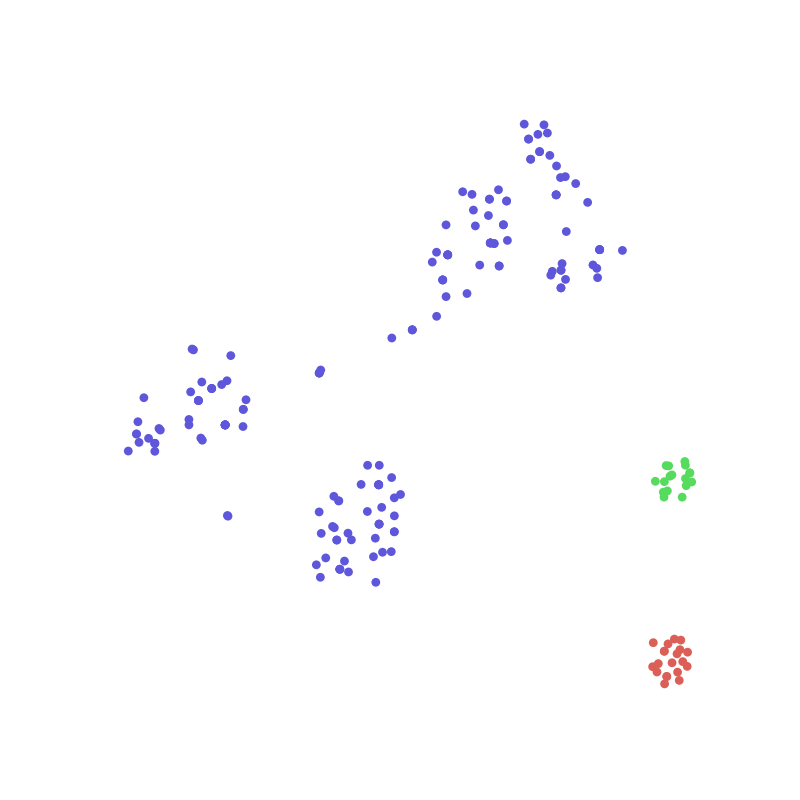
\includegraphics[scale=0.2]{tsne_viz.png}

Classification:
Why classification? 
We are able to learn clusters accurately, but the problem is that using the clusters for predictive analysis performs poorly. The reason is that clusters are diffuse and in order to predict if a graph is in a cluster or not, the arithmetic mean of all pints in the cluster is computed. Doing so, however, results in information loss and leads to inaccurate results.

Start with a set of good graphs and a restricted set of test graphs
Classification worked perfectly when we have 16-dimensional vectors for the nodes \ newline
%\includegraphics[scale=0.4]{logistic_2d.png} \newline
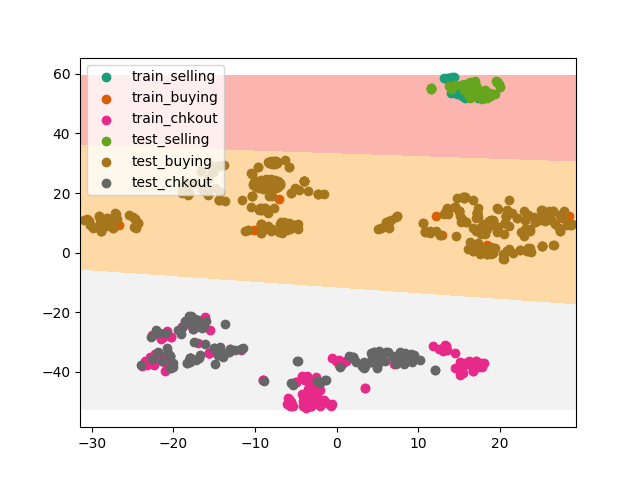
\includegraphics[scale=0.5]{test_logistic_2d.png} \newline

We split our graphs into a training set and a test set
Specifically, we used the graphs from successful executions as training graphs and those from failed interactions as test graphs
We are able to learn a logistic regression classifier that is able to predict the categories of test graph with accuracy close to 100\%
However, since not all the request paths are considered and the categories are coarse, we consider this an extended sanity check

Trace forensics: \newline
The failure here is caused by the failure of a particular service and some downstream services not being called. 
Therefore, this failure is due to the absence of one or more services.
However, all the services along the request path are alerting.
Additionally, there might also be other failures that are orthogonal to the failure which add noise to the alerts.
The hint points to a tree of services that ought to have been called, but were not. The suggestion will be to troubleshoot the service at the root of this tree first.

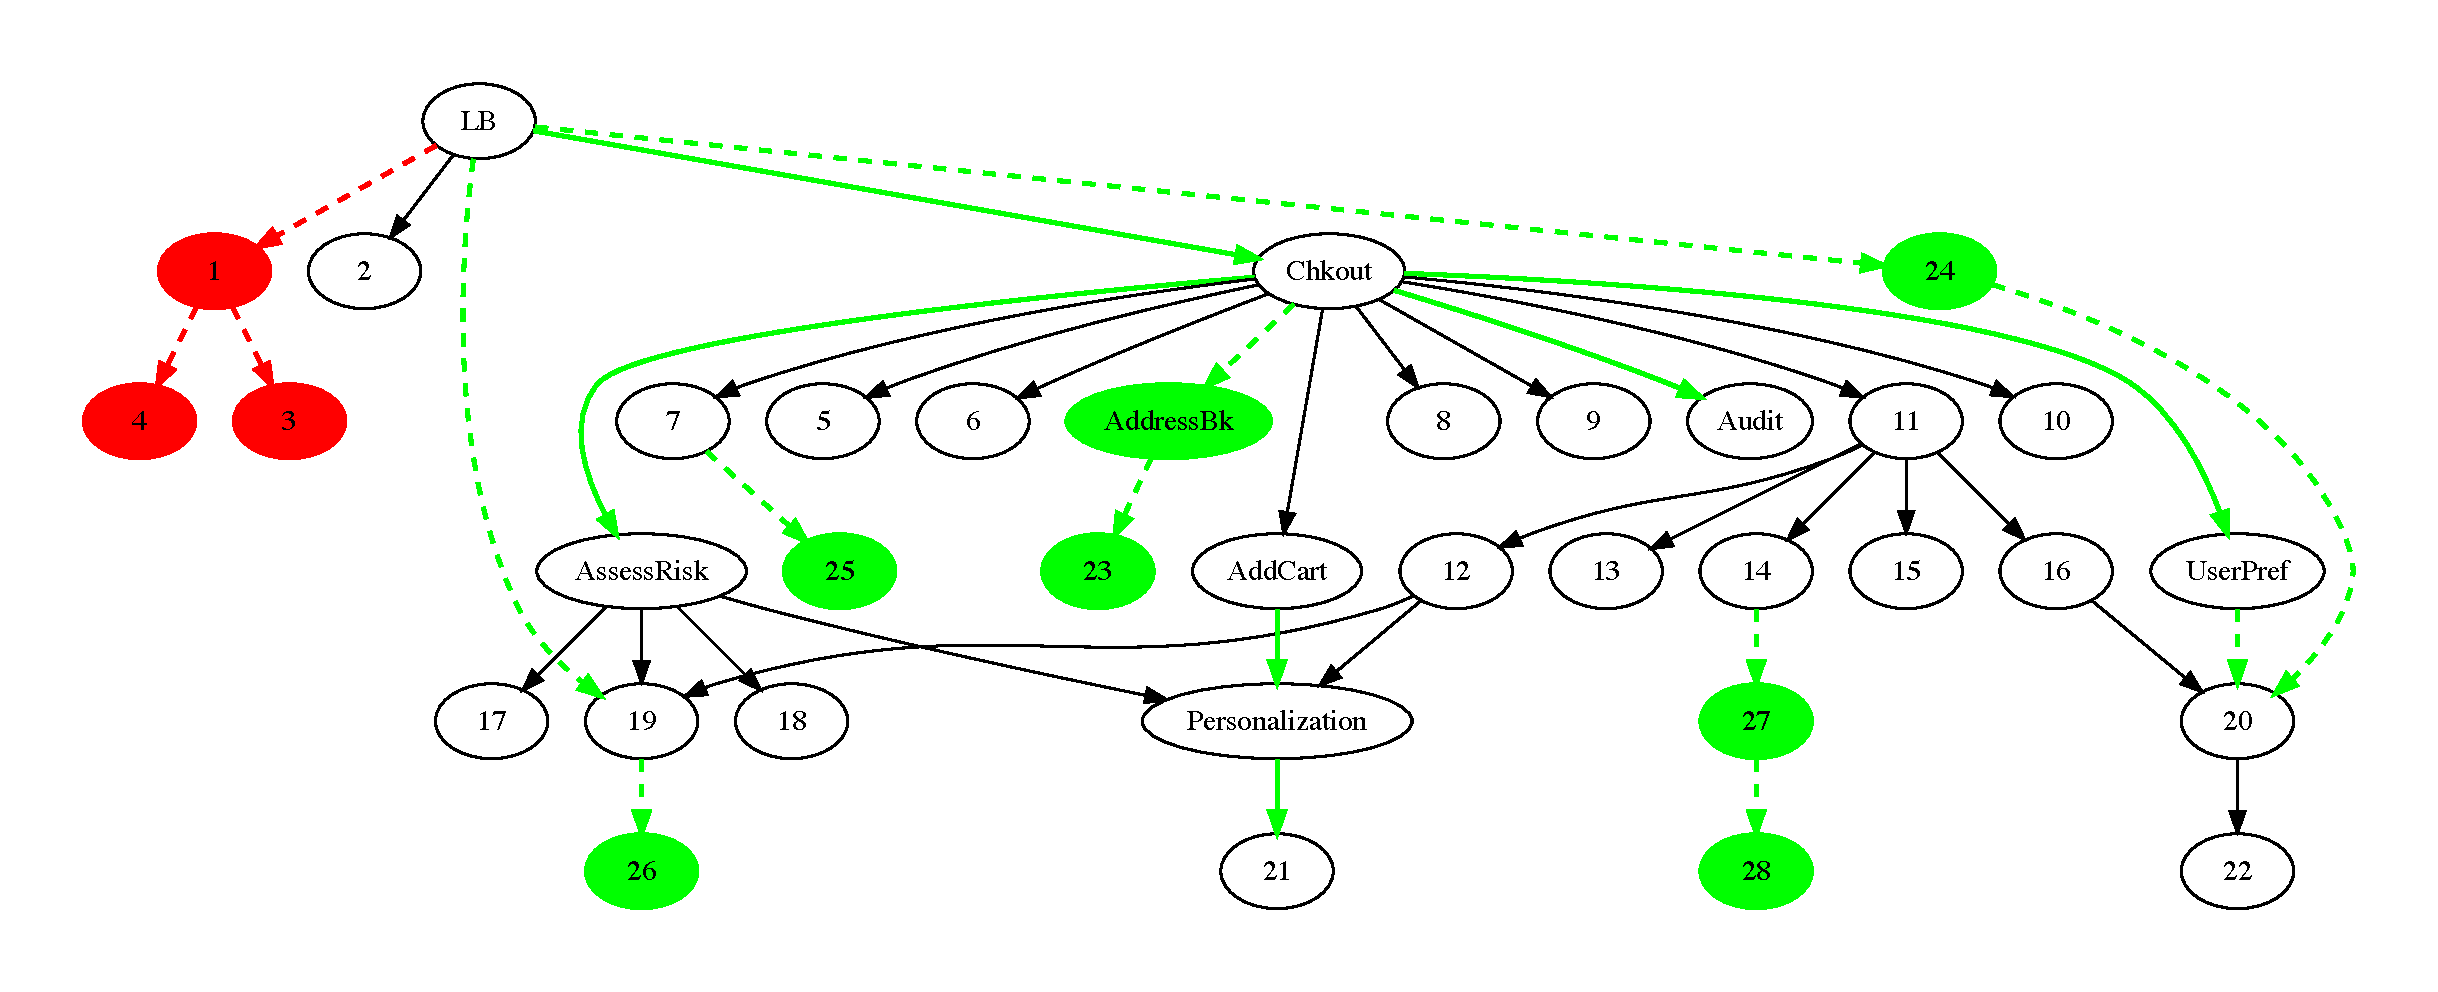
\includegraphics[width=0.5\textwidth]{anon_adrbk_repair.pdf} \newline
\kam{ There is a placeholder result graph. Services to be added are in solid green, those to be deleted in solid red. Edges to be added are in dashed green, those to be deleted are in dashed red. Solid green edges represent status needs to be successful instead of failed. Currently, there are a lot of suggestions distracting from the hint. I'm currently working to get a better completion }
